
\documentclass[a0paper,portrait]{a0poster}
\usepackage{multicol}
\usepackage{graphicx}
\usepackage{color}
\usepackage{times}
\usepackage[utf8]{inputenc}
\usepackage{amsmath}
\usepackage{url}

\setlength{\columnsep}{1cm}
\setlength{\columnseprule}{0mm}

\begin{document}
\begin{center}
    \veryHuge \textbf{From Hobby to Career: Exploring Professional eSports in Bangladesh} \par
    \vspace{1cm}
    \Huge \textbf{Author: Your Name} \par
    \vspace{1cm}
    
\includegraphics[width=0.2\linewidth]{logo.png}
\end{center}

\vspace{2cm}

\begin{multicols}{3}

\section*{Introduction}
eSports has emerged as a potential career path for many youths globally. This study explores the state of professional eSports in Bangladesh, focusing on income, challenges, and inspiration for gamers transitioning from hobbyists to professionals.

\section*{Research Objectives}
\begin{itemize}
    \item To evaluate the financial prospects in Bangladeshi eSports.
    \item To identify challenges faced by professional gamers.
    \item To understand the motivations behind choosing eSports as a career.
\end{itemize}

\section*{Methodology}
\begin{itemize}
    \item Snowball sampling to gather data.
    \item Surveys distributed to eSports players across Bangladesh.
    \item Data analysis focused on income levels, motivations, and challenges.
\end{itemize}
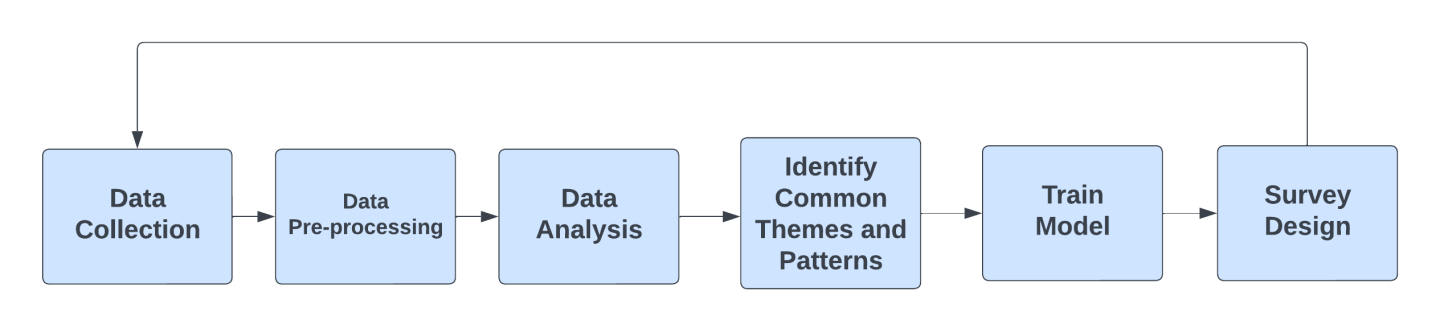
\includegraphics[width=\linewidth]{Workflow_1.png}

\section*{Findings}
\subsection*{Income Distribution Among Players}
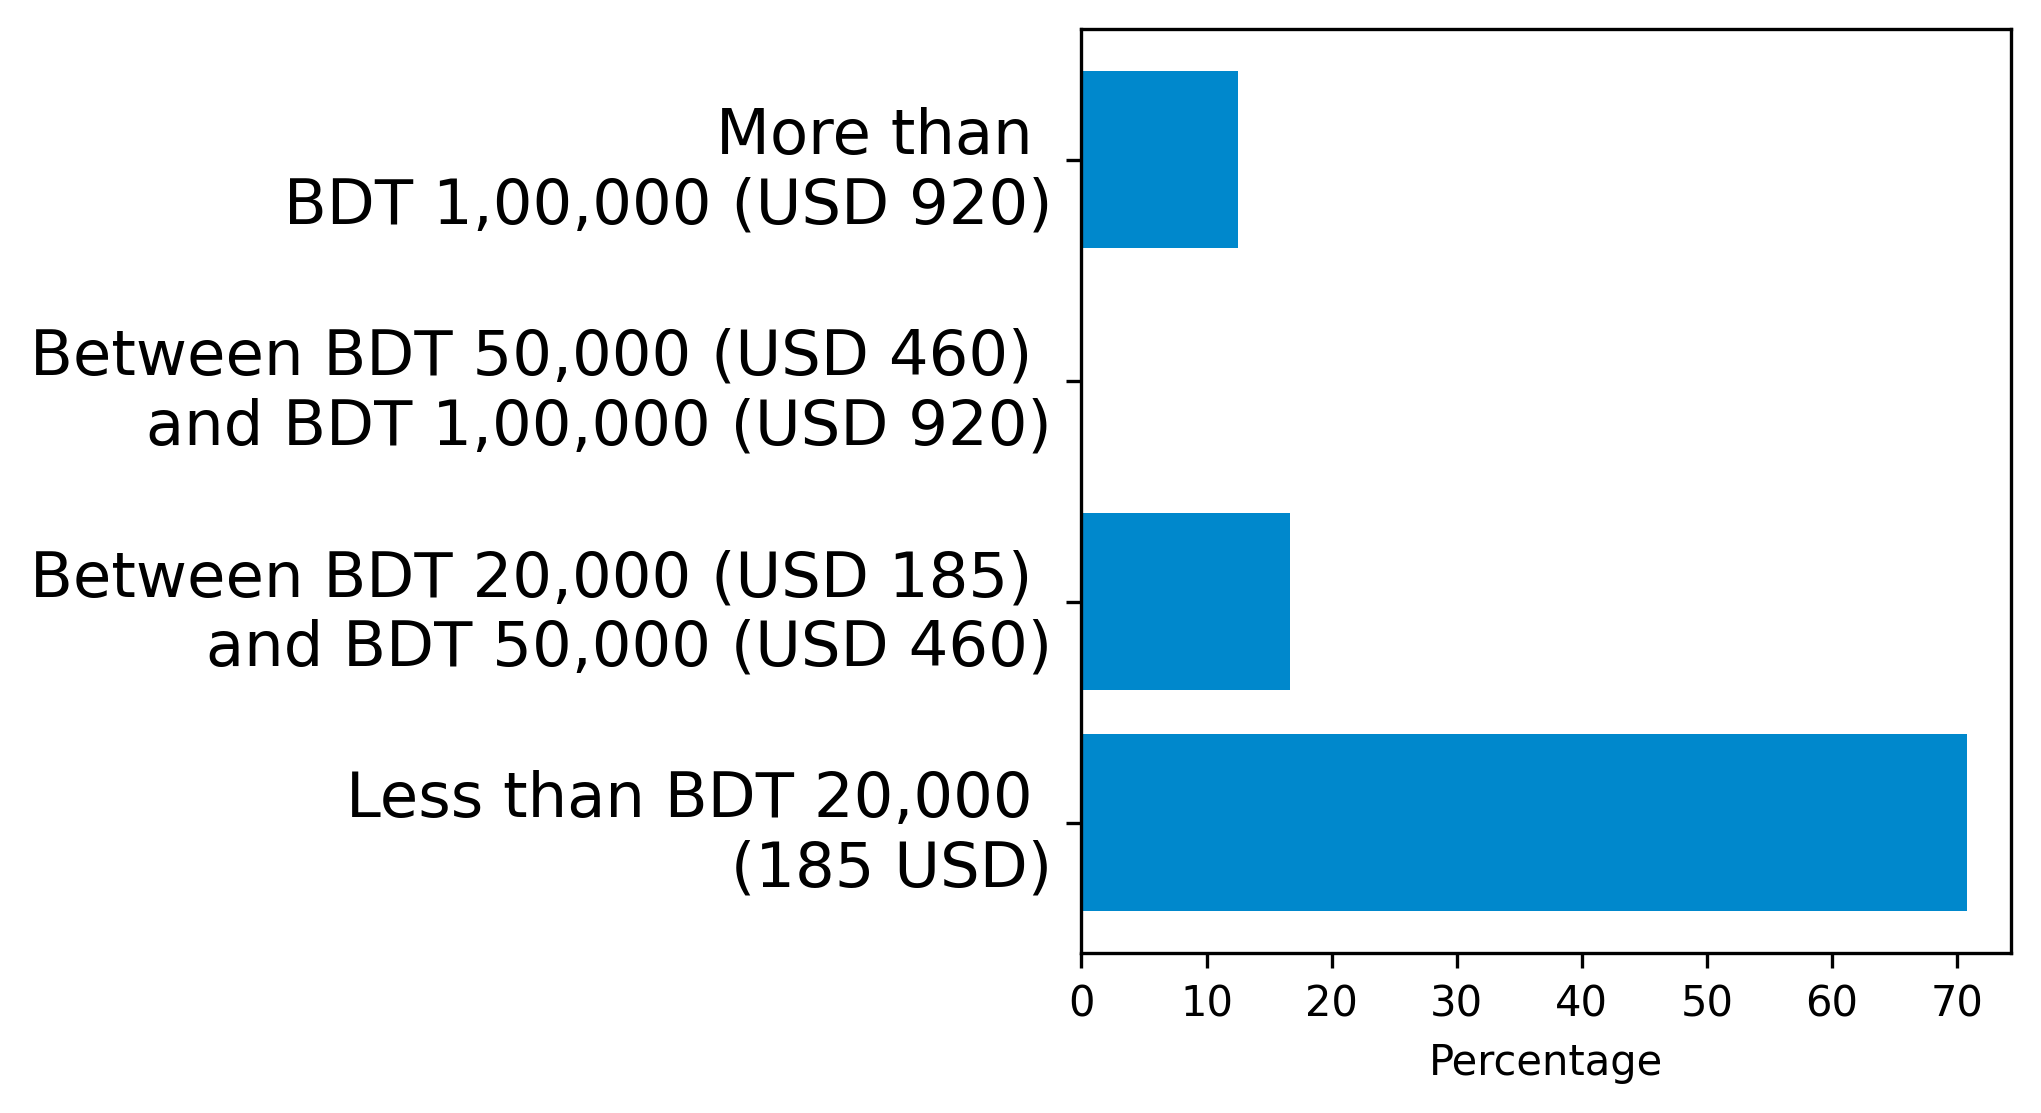
\includegraphics[width=\linewidth]{EA4.png}

\subsection*{Motivations for Choosing eSports}
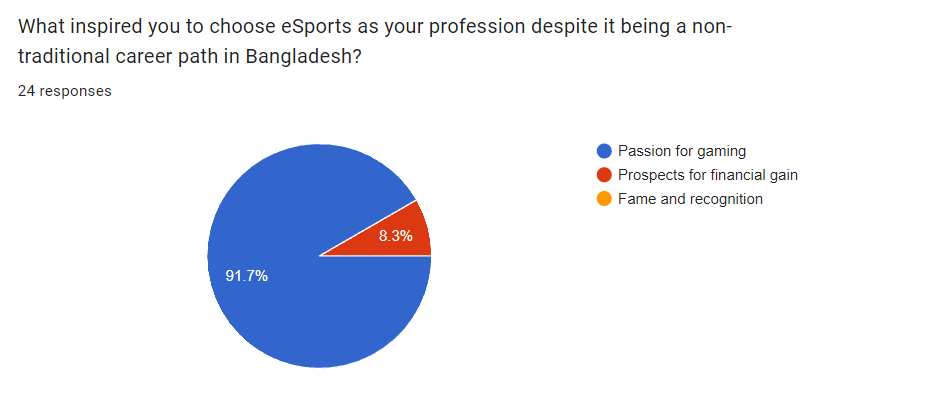
\includegraphics[width=\linewidth]{inspiration.png}

\subsection*{Challenges Faced}
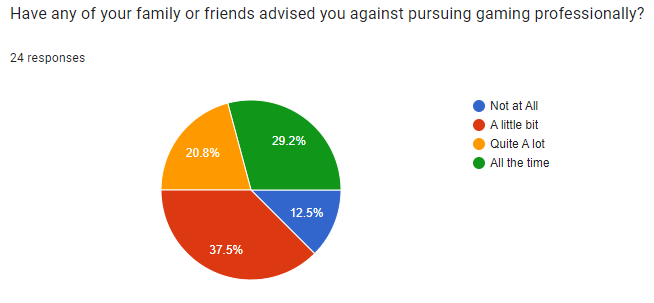
\includegraphics[width=\linewidth]{challenges.png}

\section*{Family Support and Perception}
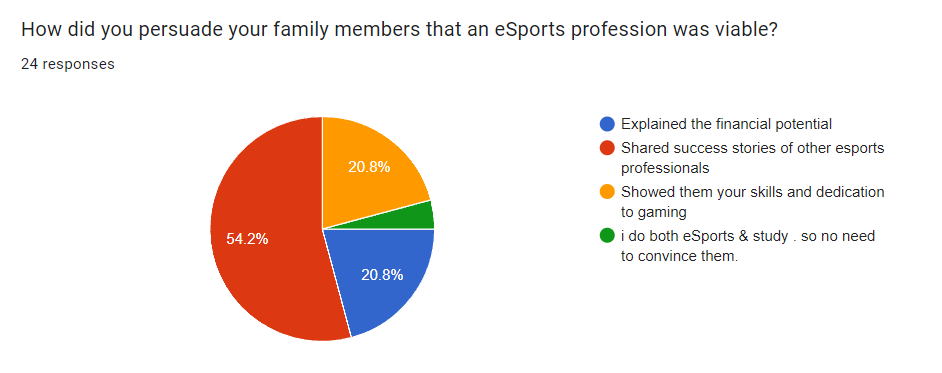
\includegraphics[width=\linewidth]{persuade your family.png}

\section*{Conclusion}
Professional eSports in Bangladesh is at a nascent stage with significant potential. Financial stability and societal acceptance remain key challenges. Passion for gaming is the primary motivator for many, showcasing a need for institutional and community support.

\section*{References}
\bibliographystyle{plain}
\bibliography{references}

\end{multicols}
\end{document}
